\chapter{Results}

%	<Paragraph> Overview of results
This chapter presents results of the $k$-{\sc Sat} execution test from the previous chapter.  We consider the results of the test and analyze the algorithm metrics. 

	\section{Algorithm metric comparison}
	
%		<Paragraph> Summary of measured metrics
This section describes the results from the simulation.  We analyze the molecular operations count for append, extract, mix, purify, splice, and split.  Presentation of actual computation time and required memory for the solution representation allow for comparison of algorithms.

The plots in this chapter use the shapes in Figure \ref{metricKey} for algorithm type.  We superimpose a line over each plot showing the percent of satisfiable $3$-CNF instances on each clause-variable ratio $\alpha$ for our test cases.

%\subsection{Split}
%%%%%%%%%%%%%%%%%%%%%%%%%%%%%%%%%
\begin{figure}[htdp]

\begin{center}

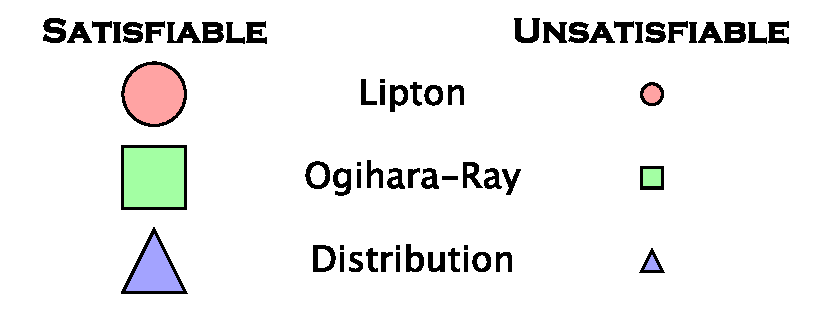
\includegraphics[width=0.7\textwidth]{./figures/key.pdf}

\caption{Key for output metrics.  Large shapes represent satisfiable instances and small shapes represent unsatisfiable instances.  Datapoints for Lipton's algorithm are represented with red circles, Ogihara and Ray's algorithm with green squares, and the Distribution algorithm with blue triangles. }
\label{metricKey}
\end{center}
\end{figure}
%%%%%%%%%%%%%%%%%%%%%%%%%%%%%%%%%

\FloatBarrier

%\subsection{Append}
%%%%%%%%%%%%%%%%%%%%%%%%%%%%%%%%%
\begin{figure}[htdp]

\reversemarginpar{
\textbf{Append} concatenates two oligonucleotides.  Figure \ref{appendFig} shows the number of appends for the naive implementations.  Figure \ref{appendFig_10} shows early termination on unsatisfiable $3$-CNF instances.   \\

The Distribution algorithm uses $O(k\cdot m)$ appends.  For unsatisfiable $k$-CNF input, the algorithm may terminate if there exist no witness candidates exist for the distribution of literals from remaining clauses. \\

Lipton's algorithm uses $\Theta(n)$ appends during the creation of a combinatorial space of $2^n$ witness candidates.\\

Ogihara and Ray's algoritm uses $O(n)$ appends.  Unsatisfiable $k$-CNF input may terminate once a conflict has been detected.\\
}

\begin{center}

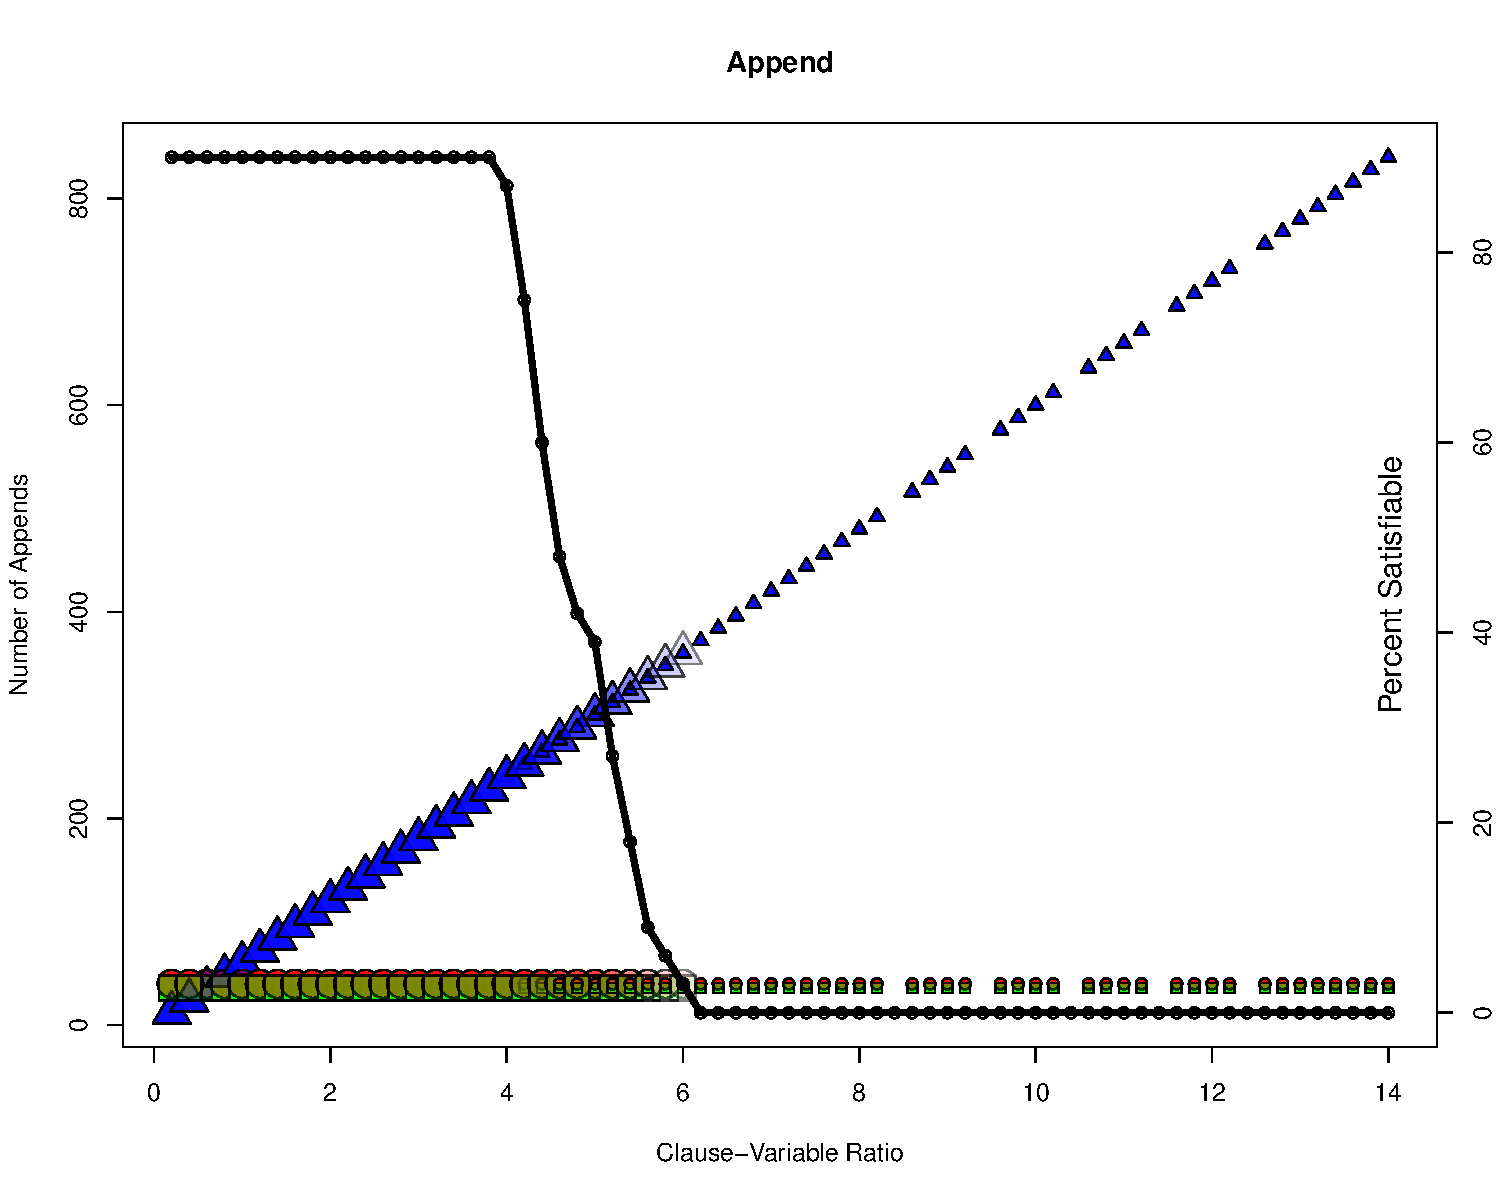
\includegraphics[width=1.1\textwidth]{./figures/metricOutput_n20/appendCount.pdf}

\caption{Clause to variable ratio $\alpha$ vs. Number of appends, with $n = 20$. }
\label{appendFig}
\end{center}
\end{figure}
%%%%%%%%%%%%%%%%%%%%%%%%%%%%%%%%%
\begin{figure}[htdp]

\begin{center}

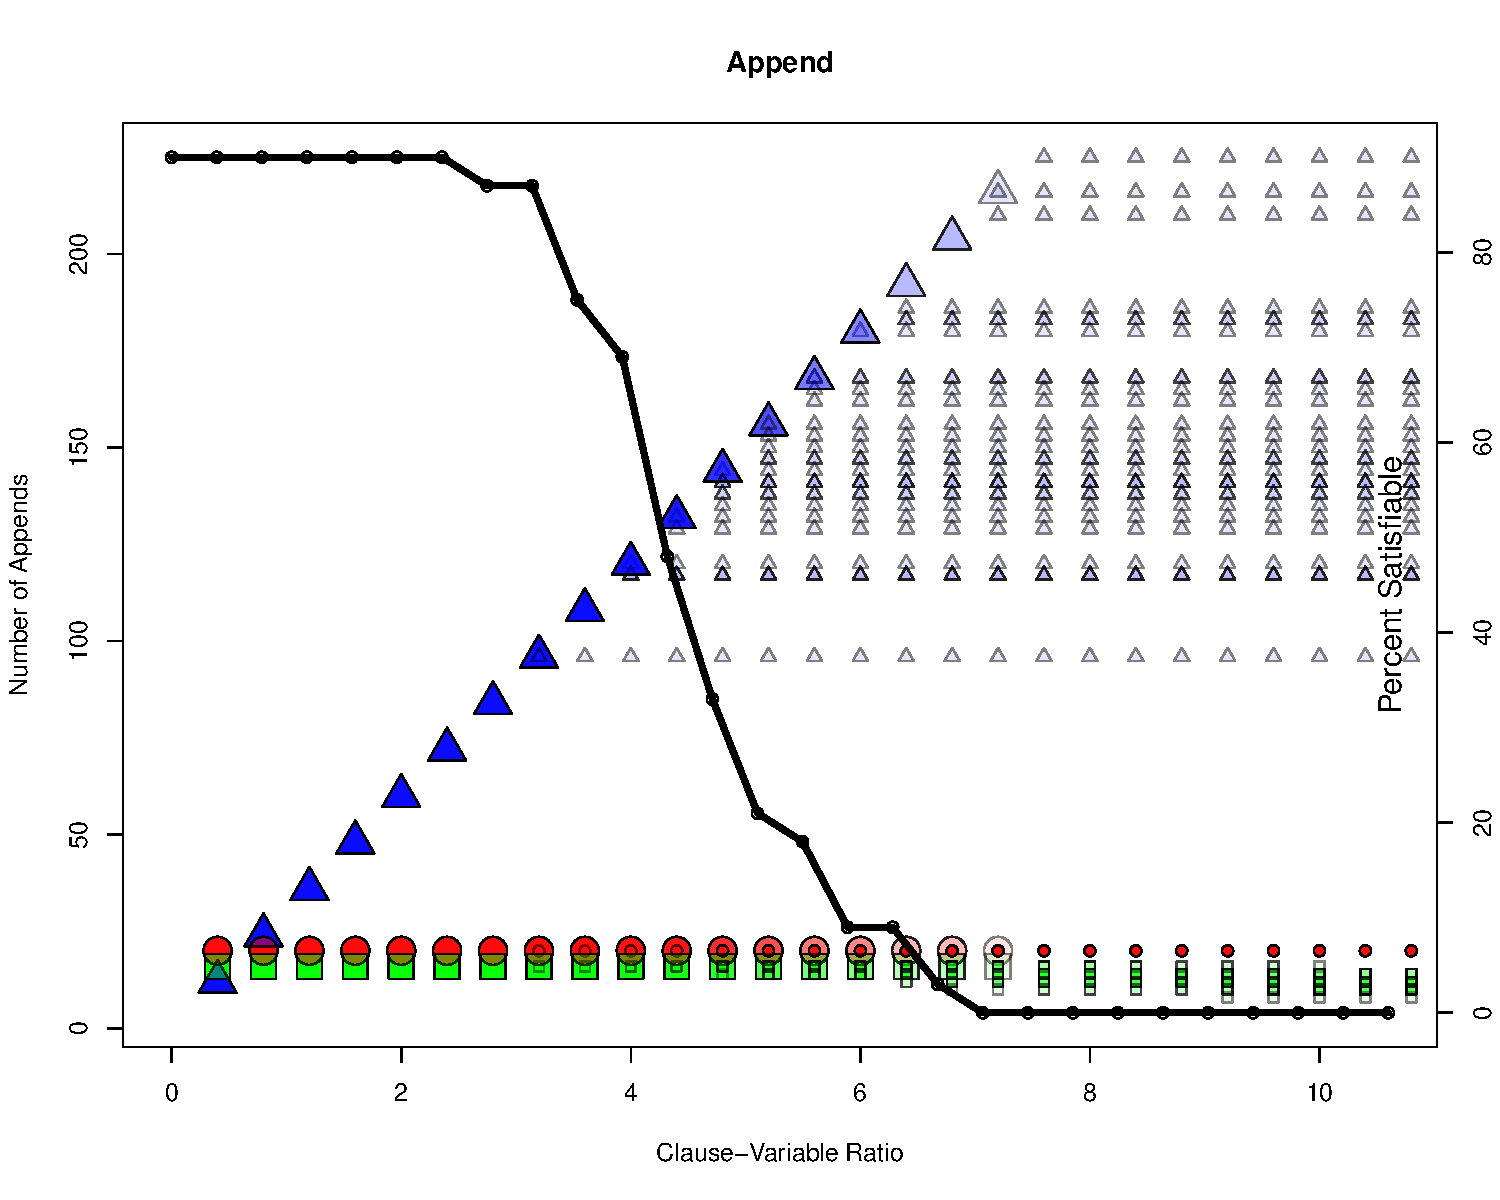
\includegraphics[width=1.1\textwidth]{./figures/metricOutput_n10/appendCount.pdf}

\caption{Clause to variable ratio $\alpha$ vs. Number of appends, with $n = 10$.  Algorithms terminate on detection of unsatisfiable input. }
\label{appendFig_10}
\end{center}
\end{figure}

%%%%%%%%%%%%%%%%%%%%%%%%%%%%%%%%%
\FloatBarrier
			
%\subsection{Extract}
%%%%%%%%%%%%%%%%%%%%%%%%%%%%%%%%%
\begin{figure}[htdp]

\reversemarginpar{

\textbf{Extract} filters oligonucleotides from a tube.  Figure \ref{extractFig} shows the number of extracts used in the naive implementations.  Figure \ref{extractFig_10} shows early termination on unsatisfiable $3$-CNF instances.   \\

Lipton's algorithm and the Distribution algorithm use $O(k\cdot m)$ extracts.  The Distribution algorithm varies a constant amount for maintaing the tubes $T_N$, $T_P$, and $T_V$.\\

Ogihara and Ray's algorithm uses $O(m)$ extracts.   Lipton's algorithm shares the same complexity from the experiments since we use $3$-CNF instances.\\

}

\begin{center}

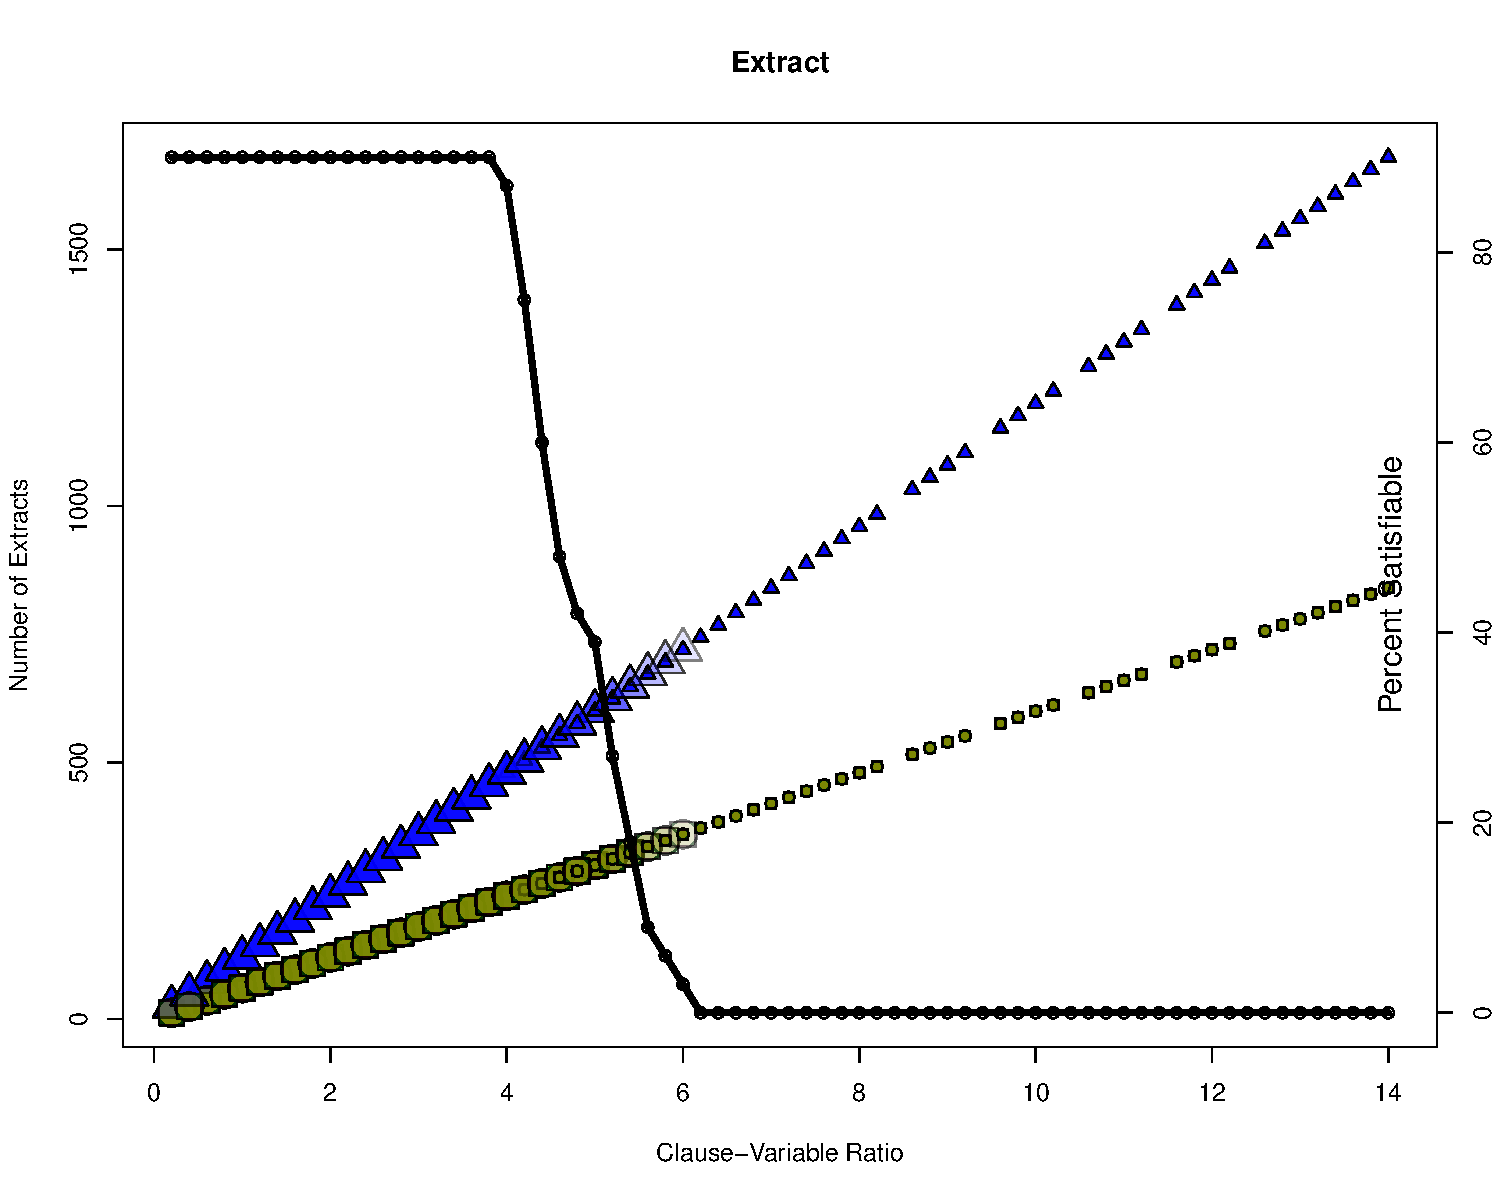
\includegraphics[width=1.1\textwidth]{./figures/metricOutput_n20/extractCount.pdf}

\caption{Clause to variable ratio $\alpha$ vs. Number of extracts, with $n= 20$. }
\label{extractFig}
\end{center}
\end{figure}
%%%%%%%%%%%%%%%%%%%%%%%%%%%%%%%%%
\FloatBarrier			
			
\begin{figure}[htdp]

\begin{center}

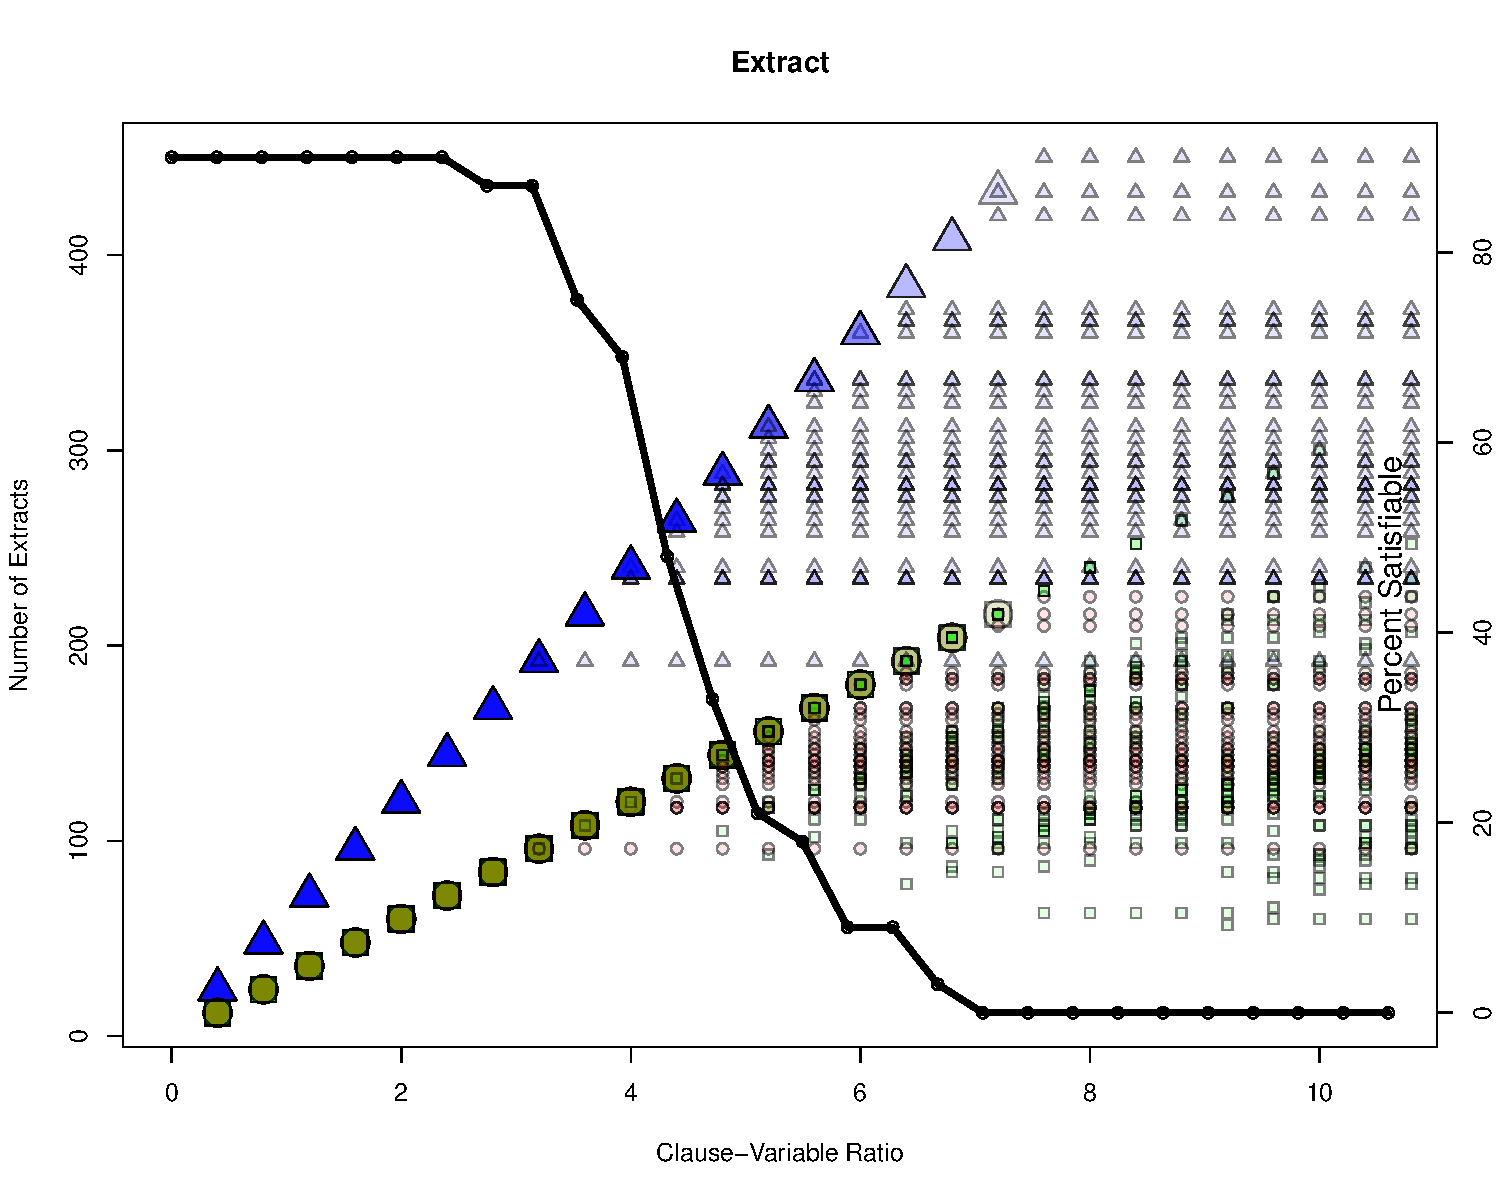
\includegraphics[width=1.1\textwidth]{./figures/metricOutput_n10/extractCount.pdf}

\caption{Clause to variable ratio $\alpha$ vs. Number of extracts, with $n = 10$.  Algorithms terminate on detection of unsatisfiable input. }
\label{extractFig_10}
\end{center}
\end{figure}

%%%%%%%%%%%%%%%%%%%%%%%%%%%%%%%%%			
			
%\subsection{Mix}
%%%%%%%%%%%%%%%%%%%%%%%%%%%%%%%%%
\begin{figure}[htdp]

\reversemarginpar{
		\textbf{Mix} combines the contents of $n$ tubes into a storage tube.  Figure \ref{mixFig} shows the number of mixes used in the naive implementations.  Figure \ref{mixFig_10} shows early termination on unsatisfiable $3$-CNF instances. \\
		
		Lipton's algorithm uses $\Theta(m(k+1)+n)$ mix operations for satisfiable $k$-CNF instances.  This includes preparing a combinatorial space with the {\sc Combinatorial Generate} subroutine.  \\
		
		The Distribution algorithm uses $O(k\cdot m)$ mixes for distributing each clause with $k$ literals into a set of witnesses satisfying each clause.  This set of witnesses get mixed into the tube satisfying all distributed clauses.\\
		
		Ogihara and Ray's algorithm expands on clauses matching in the third ordered literal.  The algorithm uses $O(m+n)$ mixes.  This includes a maximum of $m$ mixes for each clause, and $n$ mixes for extending witnesses for $\phi$.  \\

}

\begin{center}

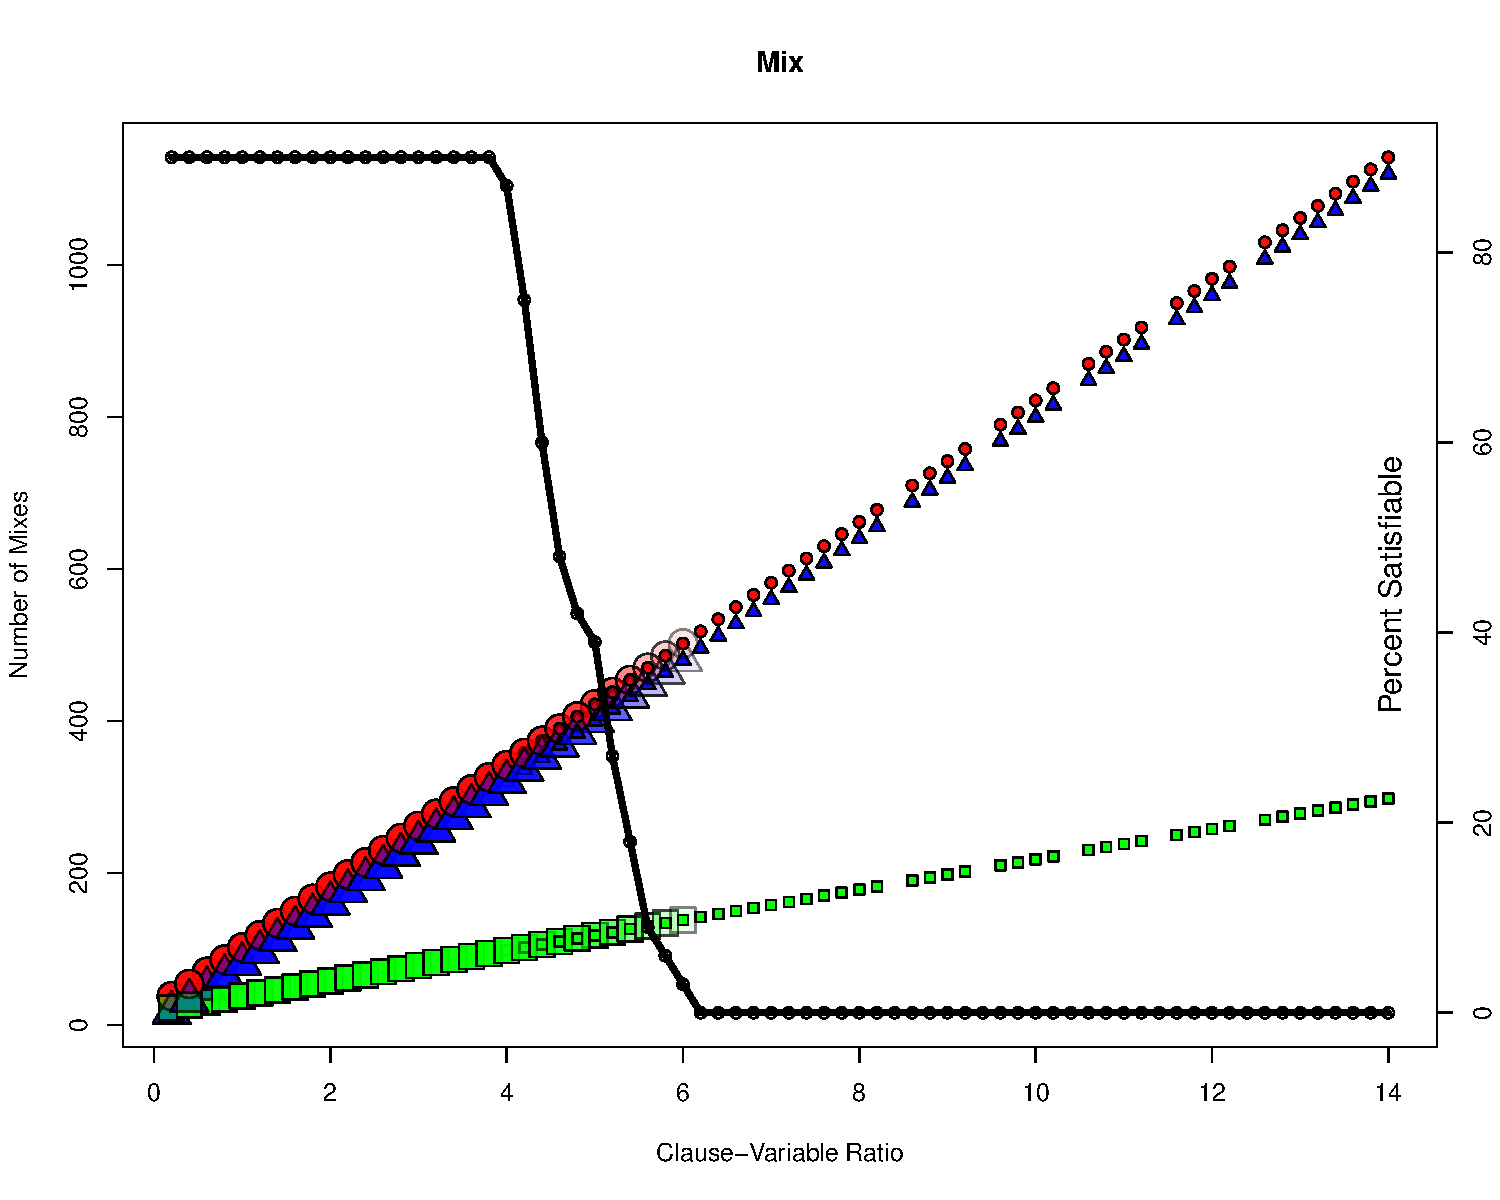
\includegraphics[width=1.1\textwidth]{./figures/metricOutput_n20/mixCount.pdf}

\caption{Clause to variable ratio $\alpha$ vs. Number of mixes, with $n = 20$.}
\label{mixFig}
\end{center}
\end{figure}

%%%%%%%%%%%%%%%%%%%%%%%%%%%%%%%%%
\begin{figure}[htdp]

\begin{center}

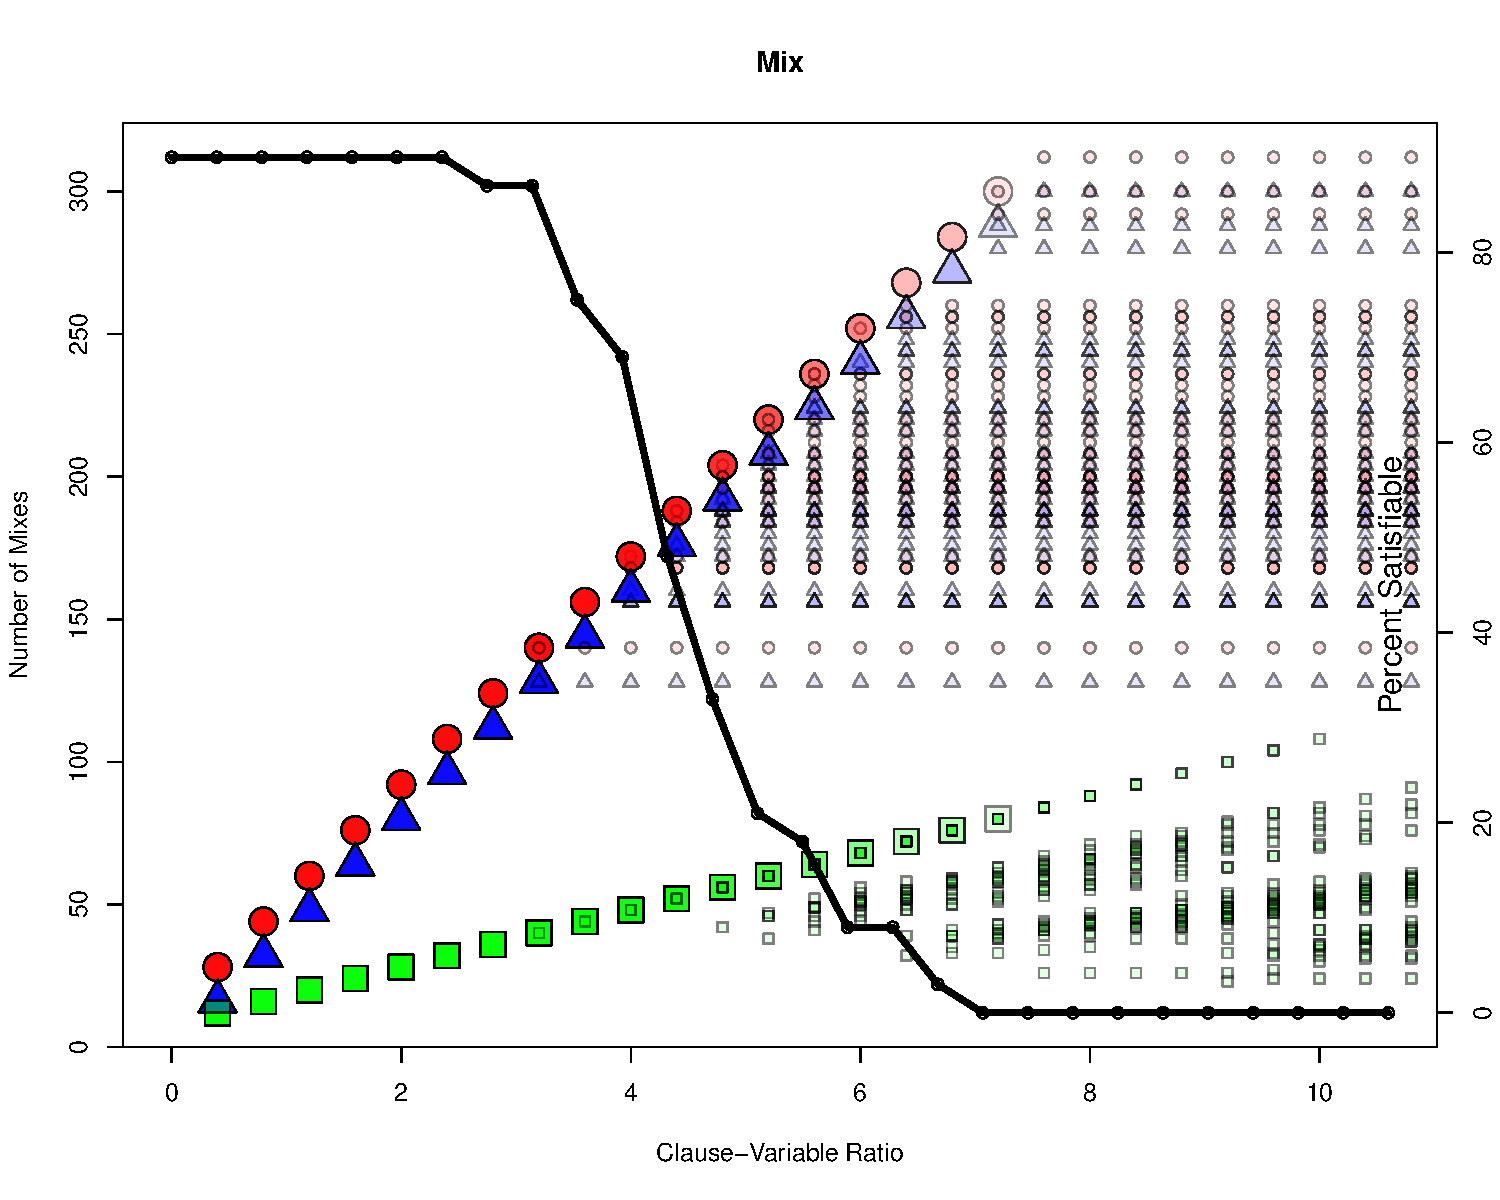
\includegraphics[width=1.1\textwidth]{./figures/metricOutput_n10/mixCount.pdf}

\caption{Clause to variable ratio $\alpha$ vs. Number of mixes, with $n = 10$.  Algorithms terminate on detection of unsatisfiable input. }
\label{mixFig_10}
\end{center}
\end{figure}

%%%%%%%%%%%%%%%%%%%%%%%%%%%%%%%%%
\FloatBarrier

%\subsection{Purify}
%%%%%%%%%%%%%%%%%%%%%%%%%%%%%%%%%
\begin{figure}[htdp]

\reversemarginpar{
\textbf{Purify} ensures a uniform distribution of each independent oligonucleotide in a tube.  Figure \ref{purifyFig} shows the number of purifications used in the naive implementations.  Figure \ref{purifyFig_10} shows early termination on unsatisfiable $3$-CNF instances. \\

Ogihara and Ray's algorithm requires $O(m+n)$ purifications.  The algorithm requires a purification for each of the $m$ clauses, and a purification for each of the $n$ variables. \\

Lipton's and the Distribution algorithms each use $O(m)$ purifications.  Each of these algorithms purify the contents on the iteration of each of the $m$ clauses.

 }

\begin{center}

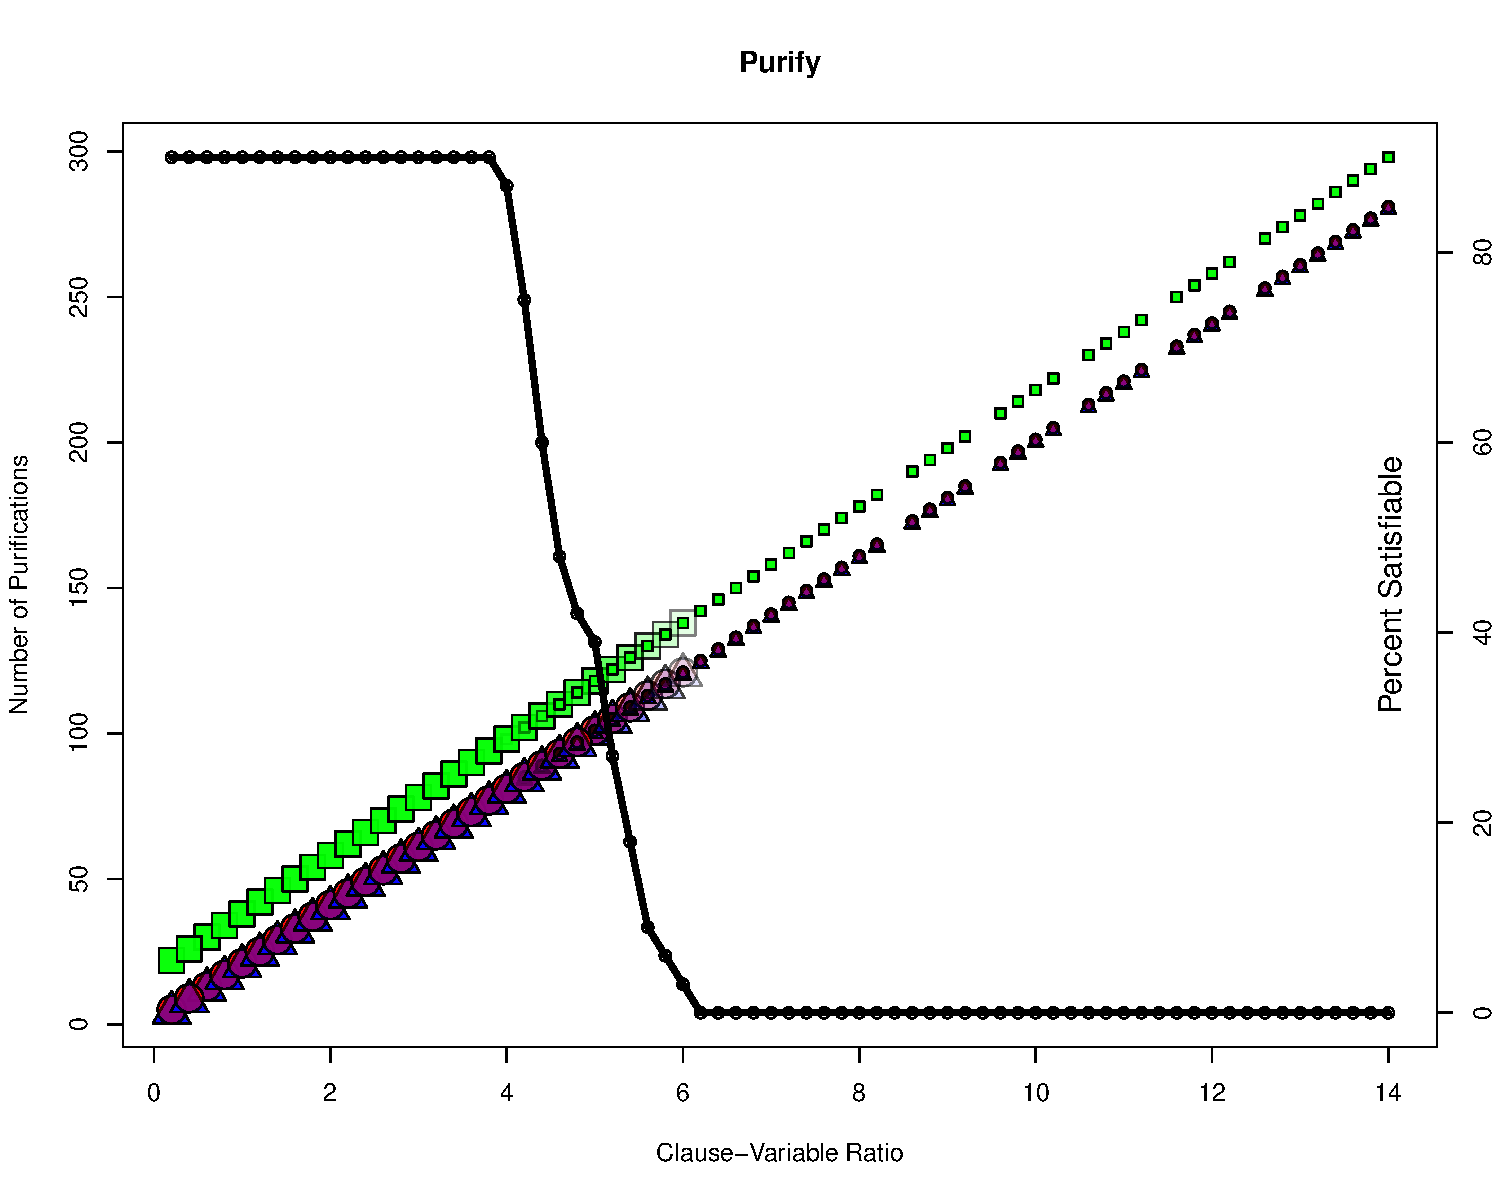
\includegraphics[width=1.1\textwidth]{./figures/metricOutput_n20/purifyCount.pdf}

\caption{Clause to variable ratio $\alpha$ vs. Number of purifications, with $n = 20$. }
\label{purifyFig}
\end{center}
\end{figure}
%%%%%%%%%%%%%%%%%%%%%%%%%%%%%%%%%

\begin{figure}[htdp]

\begin{center}

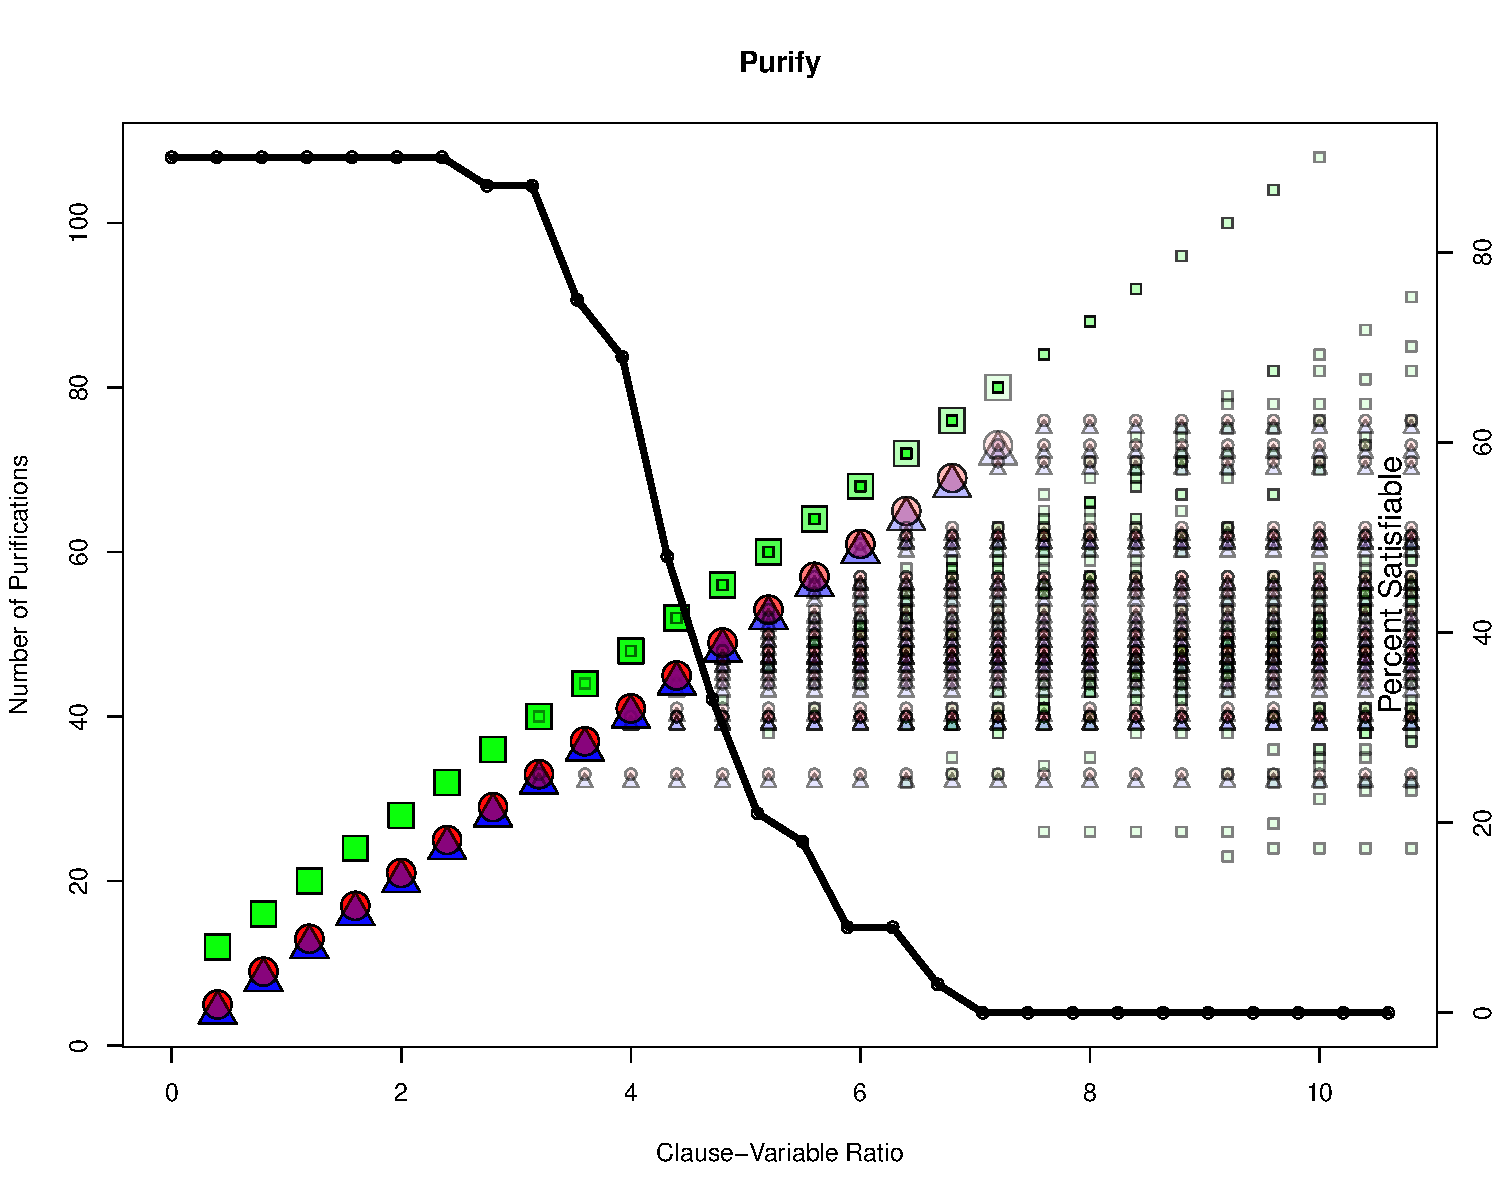
\includegraphics[width=1.1\textwidth]{./figures/metricOutput_n10/purifyCount.pdf}

\caption{Clause to variable ratio $\alpha$ vs. Number of purifications, with $n = 10$.  Algorithms terminate on detection of unsatisfiable input. }
\label{purifyFig_10}
\end{center}
\end{figure}

%%%%%%%%%%%%%%%%%%%%%%%%%%%%%%%%%
\FloatBarrier


%\subsection{Split}
%%%%%%%%%%%%%%%%%%%%%%%%%%%%%%%%%
\begin{figure}[htdp]

\reversemarginpar{

\textbf{Split} portions a tube into two exact tubes.  Figure \ref{splitFig} shows the number of splits used in the naive implementations.  Figure \ref{splitFig_10} shows early termination on unsatisfiable $3$-CNF instances. \\

The Distribution algorithm uses $O(k \cdot m)$ splits.  The split operation occurs on each of the $m$ clauses of a $k$-CNF instance.\\

Lipton's algorithm uses $\Theta(n)$ splits during the creation of a combinatorial space of $2^n$ witness candidates with {\sc Combinatorial Generate}.\\

Ogihara and Ray's algorithm uses $O(n)$ splits.  The algorithm requires a copy of witness candidates in the tubes ($T_P$ and $T_N$).  The tubes $T_P$ and $T_N$ extend with positive and negative literal assignments. 

 }

\begin{center}

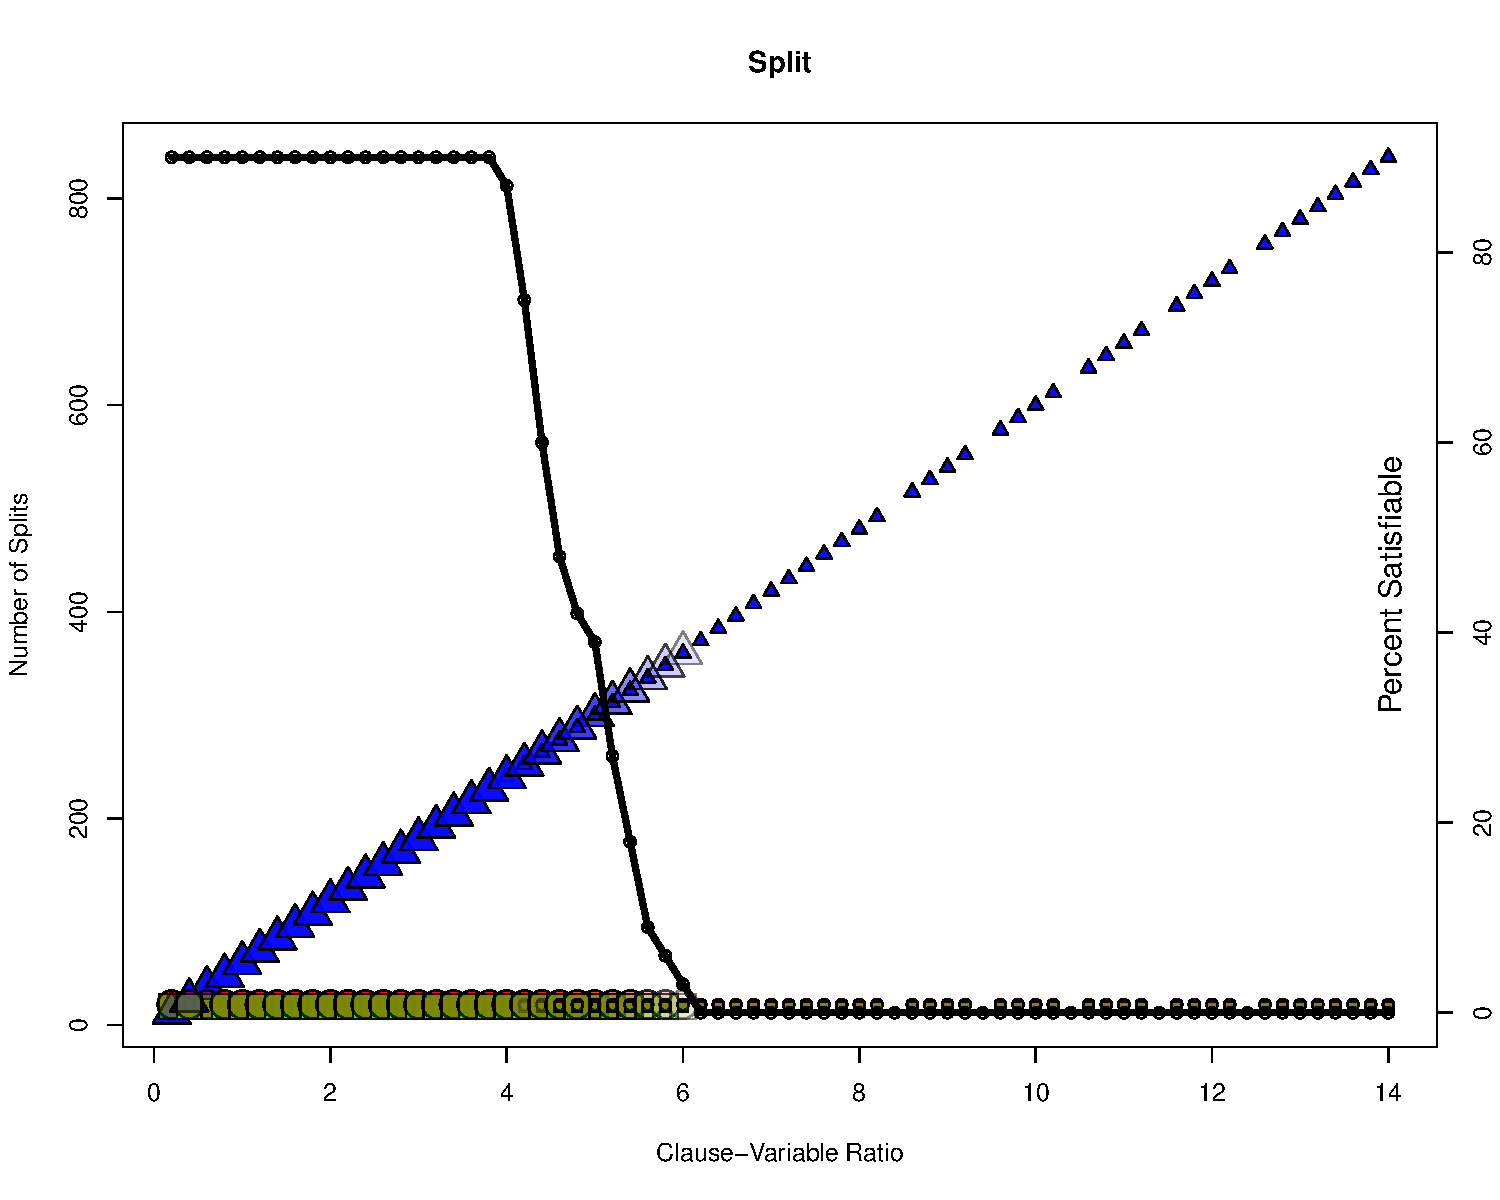
\includegraphics[width=1.1\textwidth]{./figures/metricOutput_n20/splitCount.pdf}

\caption{Clause to variable ratio $\alpha$ vs. Number of splits, with $n = 20$. }
\label{splitFig}
\end{center}
\end{figure}
%%%%%%%%%%%%%%%%%%%%%%%%%%%%%%%%%
\begin{figure}[htdp]

\begin{center}

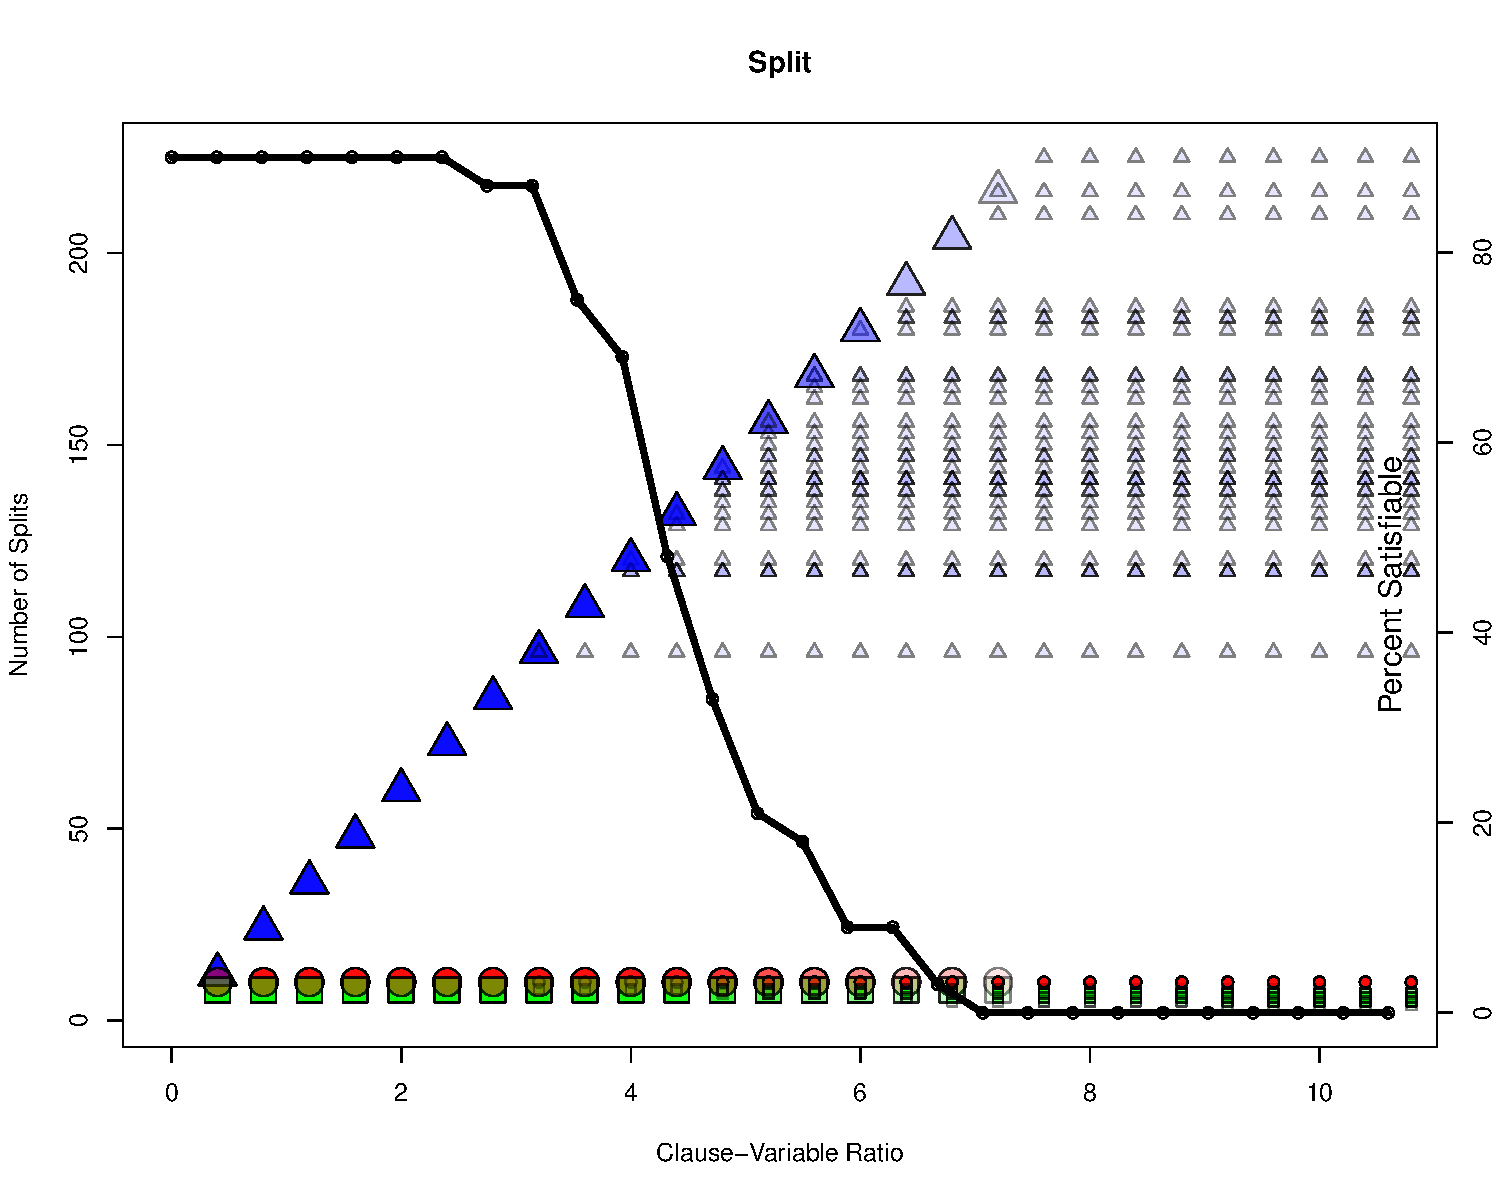
\includegraphics[width=1.1\textwidth]{./figures/metricOutput_n10/splitCount.pdf}

\caption{Clause to variable ratio $\alpha$ vs. Number of splits, with $n = 10$.  Algorithms terminate on detection of unsatisfiable input. }
\label{splitFig_10}
\end{center}
\end{figure}

%%%%%%%%%%%%%%%%%%%%%%%%%%%%%%%%%

\FloatBarrier

			
%\subsection{Time}
%%%%%%%%%%%%%%%%%%%%%%%%%%%%%%%%%
\begin{figure}[htdp]

\reversemarginpar{
\textbf{Time} measures algorithm execution time in seconds.  Figure \ref{timeFig} shows the execution time in seconds used in the naive implementations.  Figure \ref{timeFig_10} shows early termination on unsatisfiable $3$-CNF instances. \\

Ogihara and Ray's algorithm requires the least amount of time.  The algorithm takes the greatest amount of time for under-constrained instances (causing a large number of witnesses to be generated).   Less pruning occurs in over-constrained instances, reducing the execution time of test instances.\\

Lipton's algorithm executes in exponential time $\alpha \approx [4.0, 6.0]$ (the phase transition region for 3-{\sc Sat}) taking the longest.\\

The Distribution algorithm executes in exponential time, and performs better than Lipton's algorithm for low conflict ratios.  Instances take the longest from $\alpha \approx [4.0, 6.0]$ (in the $3$-{\sc Sat} phase-transition region).
}

\begin{center}

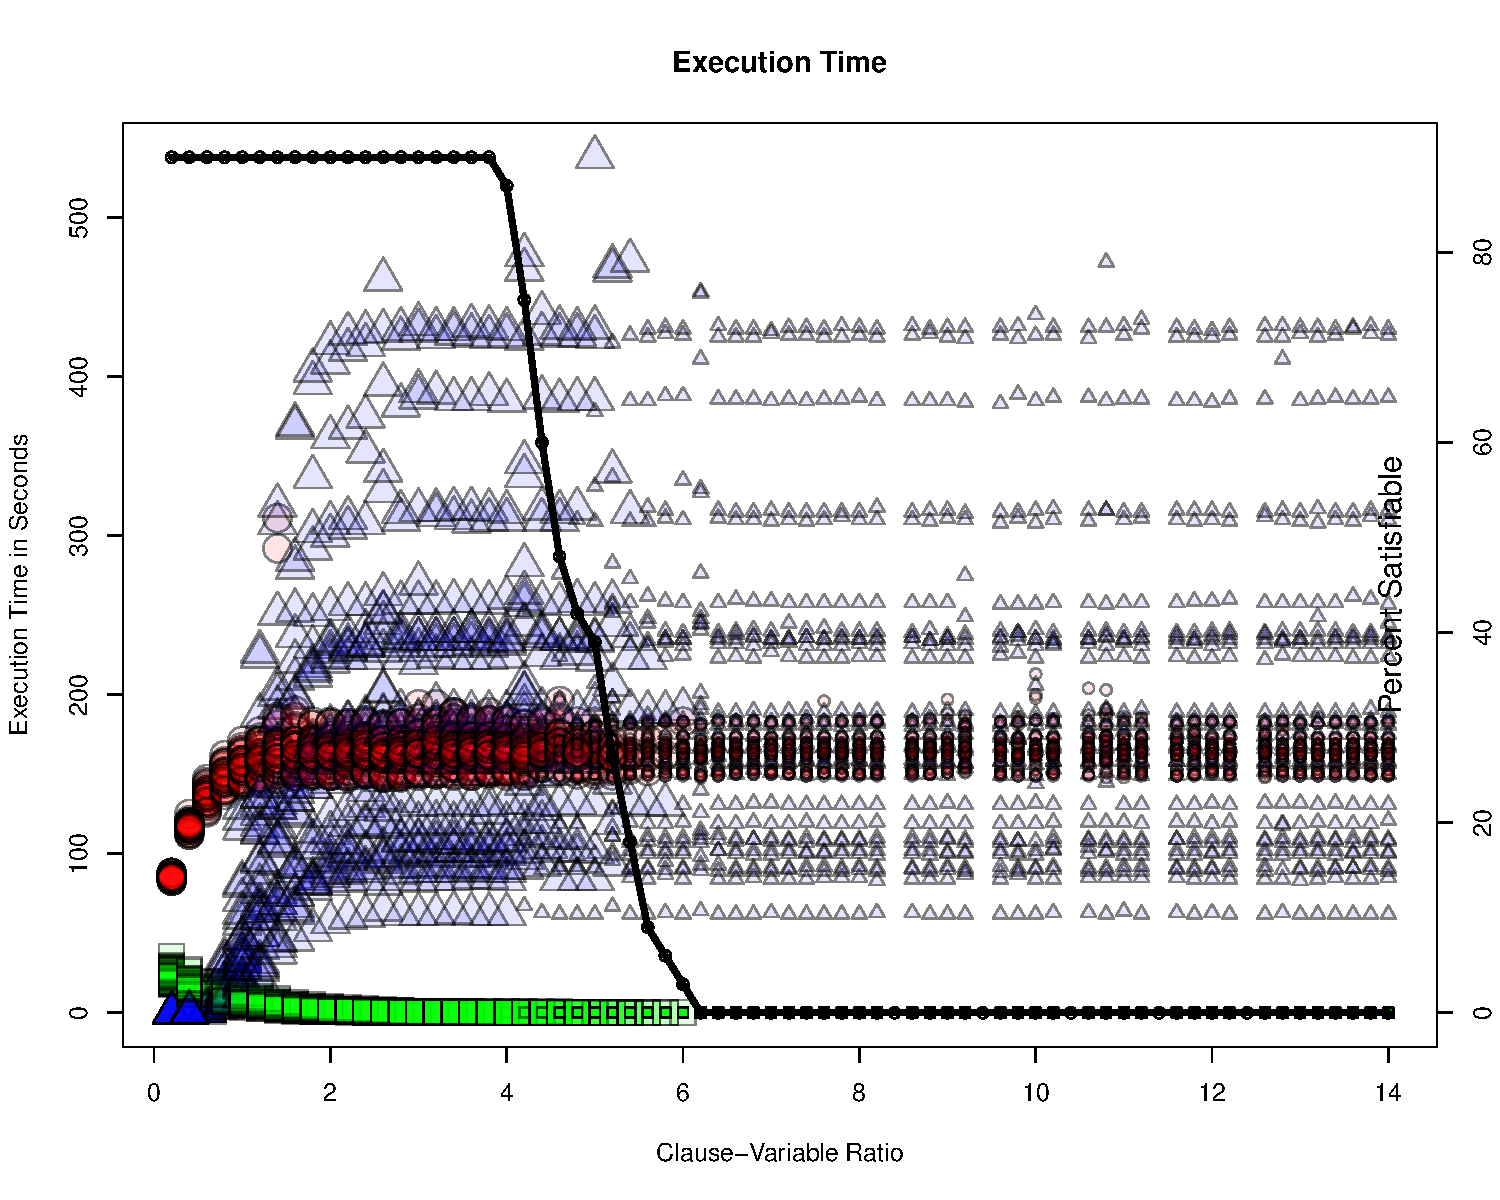
\includegraphics[width=1.1\textwidth]{./figures/metricOutput_n20/executionTime.pdf}

\caption{Clause to variable ratio $\alpha$ vs. execution time in seconds, with $n = 20$. }
\label{timeFig}
\end{center}
\end{figure}

%%%%%%%%%%%%%%%%%%%%%%%%%%%%%%%%%
\begin{figure}[htdp]

\begin{center}

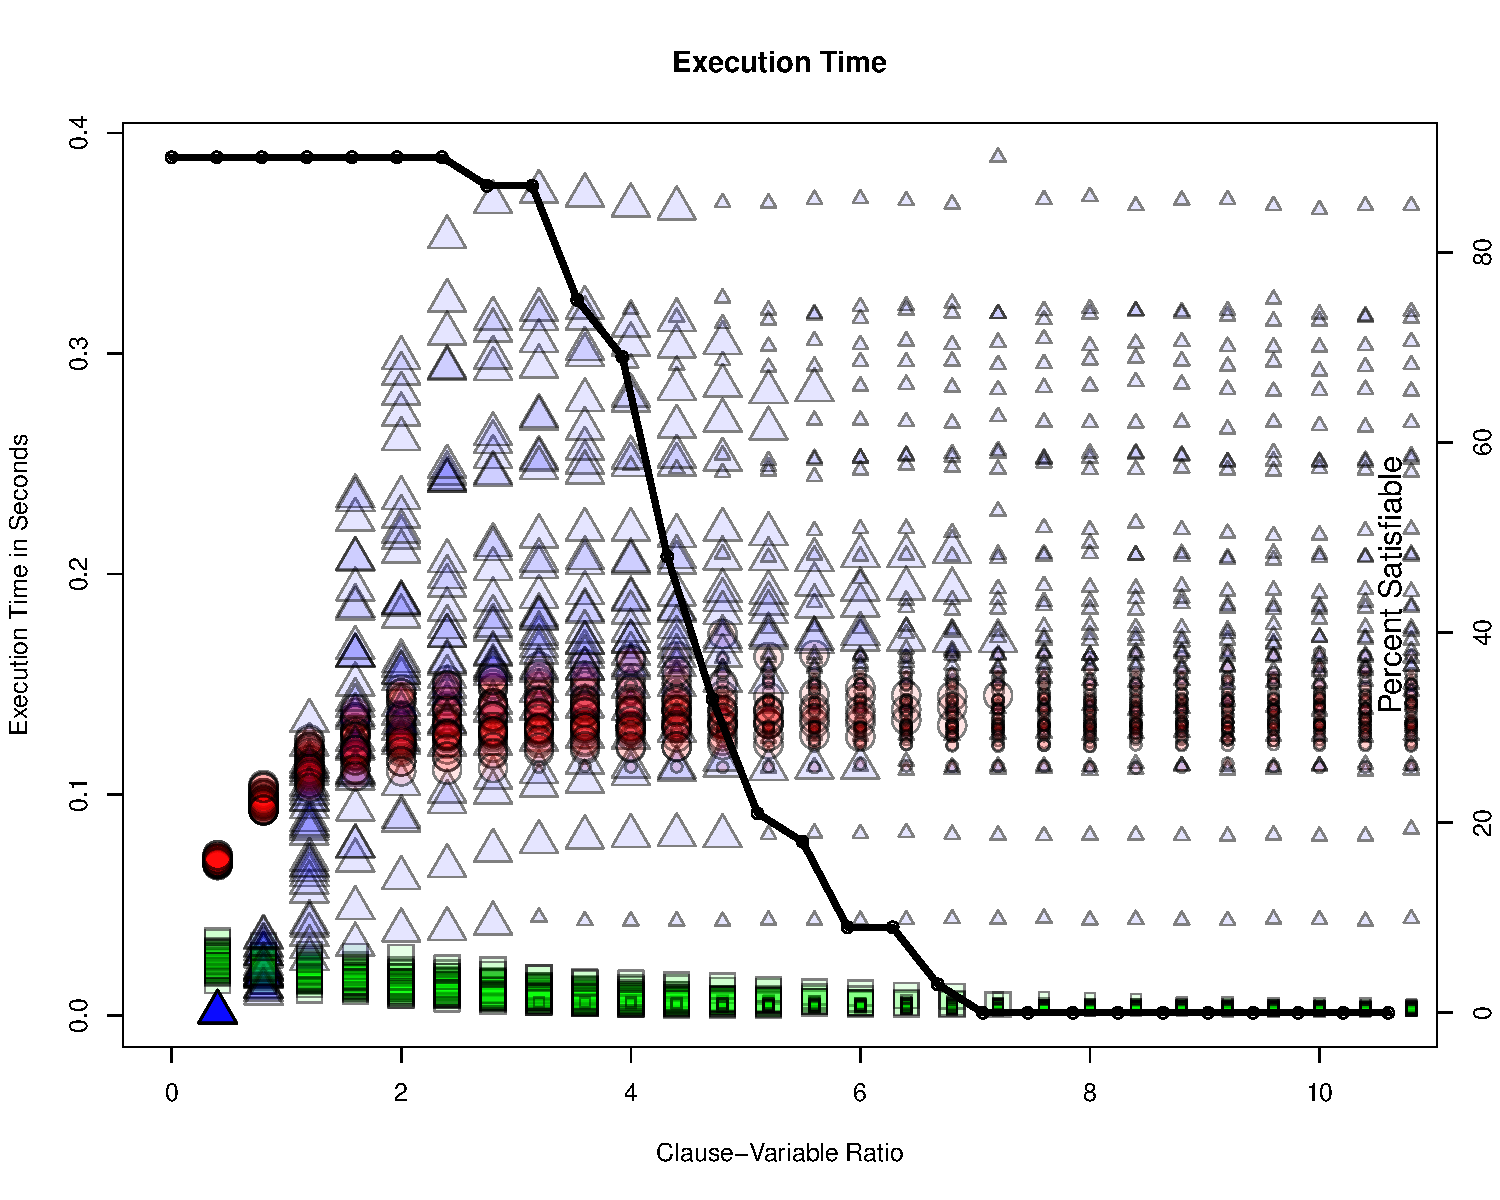
\includegraphics[width=1.1\textwidth]{./figures/metricOutput_n10/executionTime.pdf}

\caption{Clause to variable ratio $\alpha$ vs. Number of splits, with $n = 10$.  Algorithms terminate on detection of unsatisfiable input. }
\label{timeFig_10}
\end{center}
\end{figure}

%%%%%%%%%%%%%%%%%%%%%%%%%%%%%%%%%
\FloatBarrier
			
%\subsection{Solution space}
%%%%%%%%%%%%%%%%%%%%%%%%%%%%%%%%%
\begin{figure}[htdp]

\reversemarginpar{
\textbf{Memory} measures witness footprint in Bytes.  Figure \ref{memoryFig} shows the satisfiable instance witness memory.  Figure \ref{memoryFigDetail} shows a detailed view of Figure \ref{memoryFig} from $\alpha = [3,6]$.\\

Lipton's and Ogihara and Ray's algorithms share the same solution footprint.\\

The Distribution algorithm contains a larger solution footprint after the trivially satisfiable instances with $\alpha \approx [0.2, 1.0)$.  The space contains a set of over-constrained assignments from $\alpha \approx [1.0, 4.0]$.  \\

Each {\sc Satisfiability} instance has a constrained solution space during the phase-transition region.  We scale the axis in Figure \ref{memoryFig} to observe only satisfiable instances.
}

\begin{center}

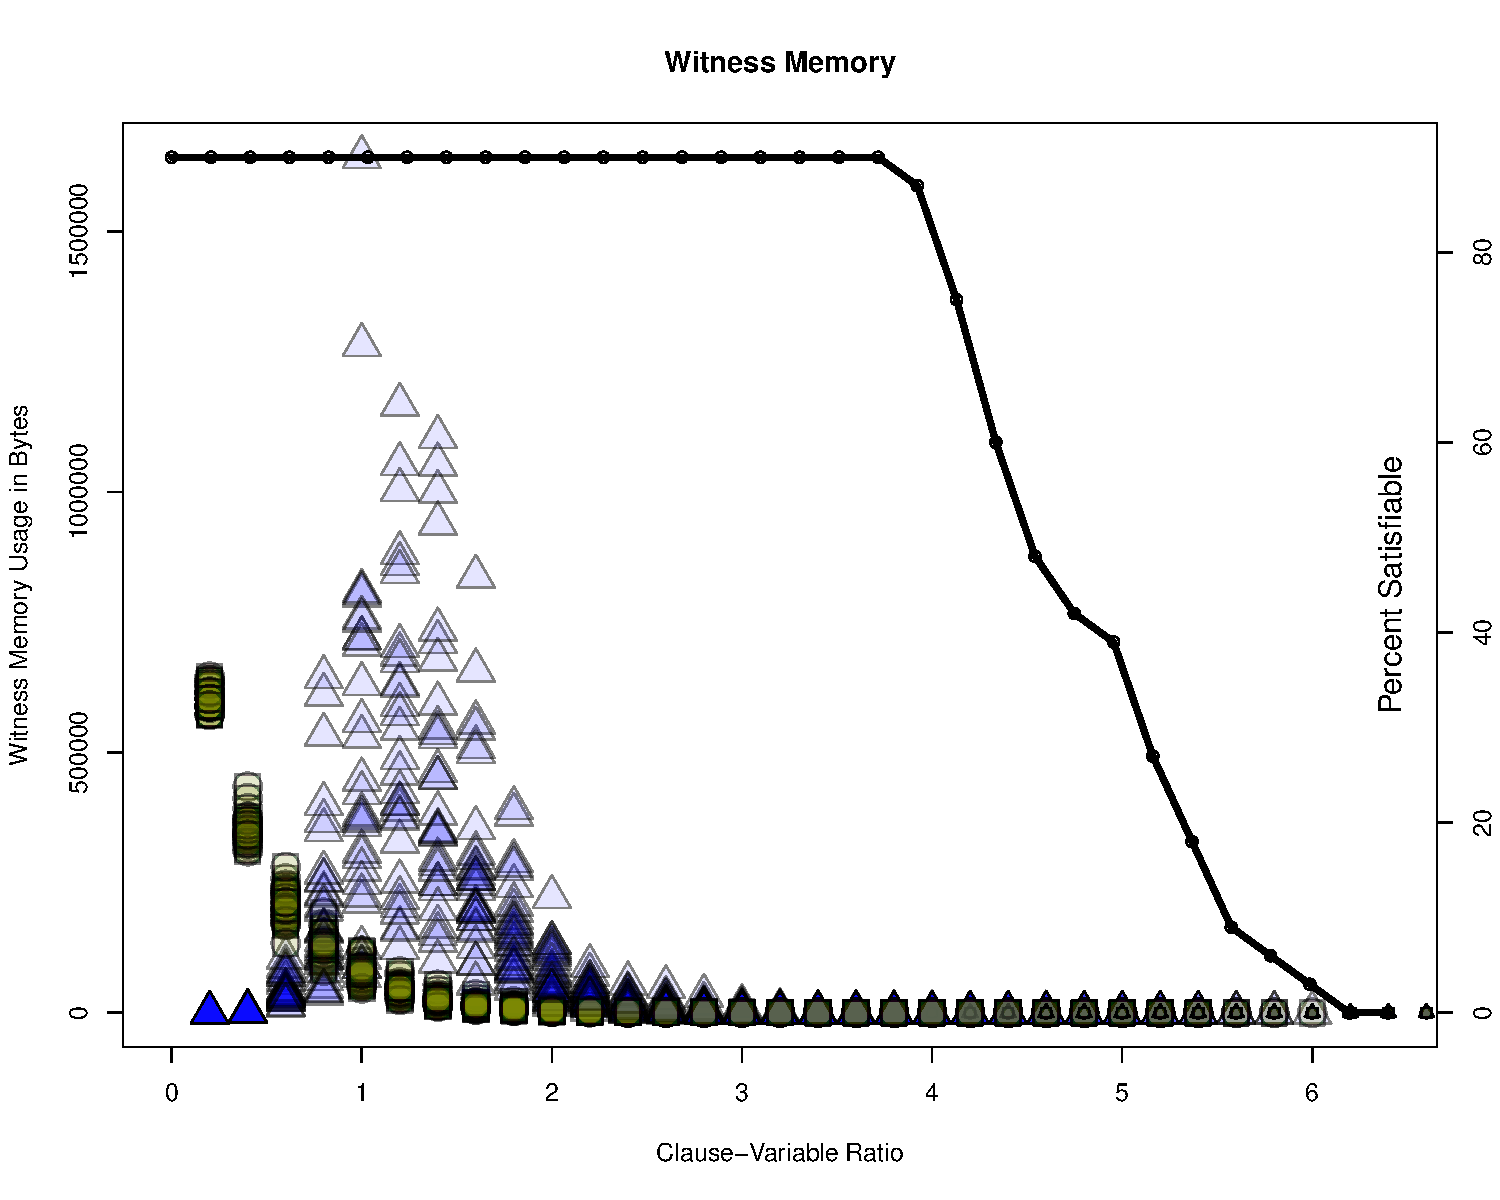
\includegraphics[width=1.1\textwidth]{./figures/plotImage/memory0-6_2.pdf}

\caption{Clause to variable ratio $\alpha$ vs. satisfiable solution footprint in Bytes, with $n = 20$. }
\label{memoryFig}
\end{center}
\end{figure}


\begin{figure}[htdp]
\begin{center}

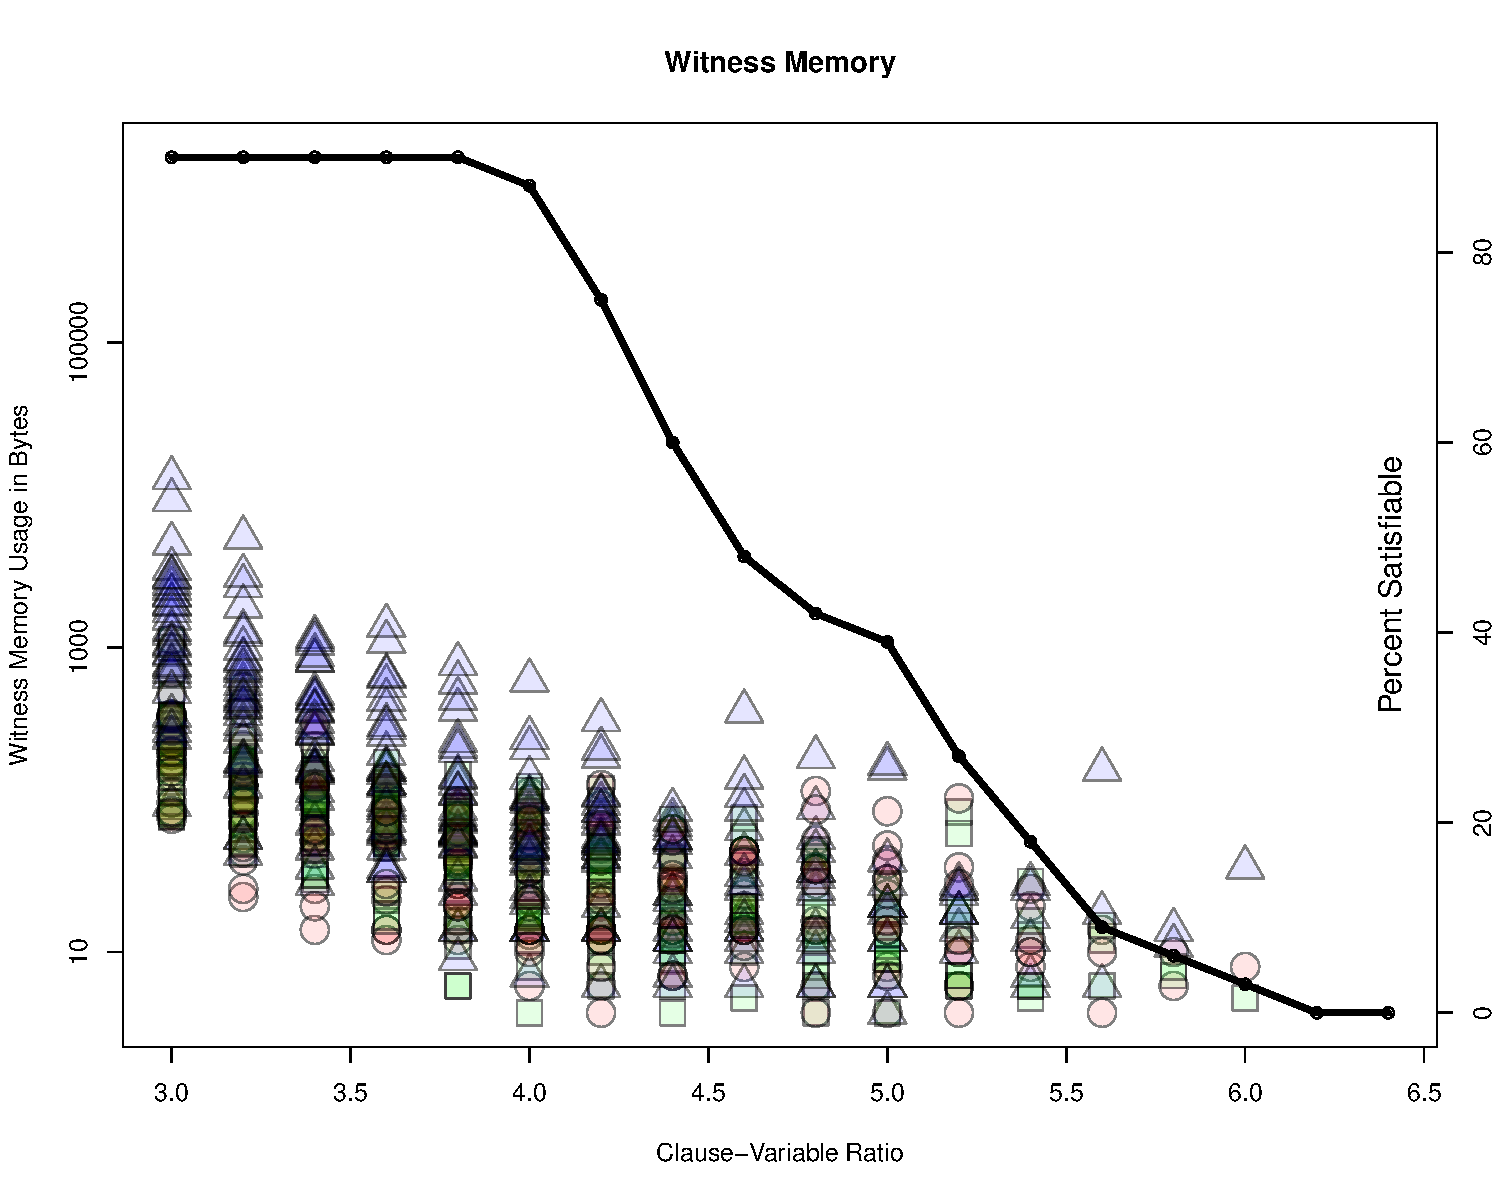
\includegraphics[width=1.1\textwidth]{./figures/plotImage/memory3-6_2.pdf}

\caption{Detailed view of Figure \ref{memoryFig} from $\alpha = [3,6]$. }
\label{memoryFigDetail}
\end{center}
\end{figure}

%%%%%%%%%%%%%%%%%%%%%%%%%%%%%%%%%

\FloatBarrier

	\section{Summary of Molecular Algorithms}

		Table \ref{timeComplexityMolecularOperators} shows a comparison of the molecular operators of the algorithms under test.  Once the solution space $T_S = \emptyset$ the algorithms can terminate.  This provides the upper bounds for execution of various $k$-CNF instances.  
		
		\begin{table}[htdp]
				\caption{Time complexity of molecular operators for each of the molecular algorithms.}
				\begin{center}
				\begin{tabular}{|c|c|c|c|c|}
					\hline
					\textbf{ Operator} & {\sc Combinatorial Generate} & {\sc Lipton}           & {\sc Ogihara-Ray}  & {\sc Distribution} \\ \hline
					mix	               & $\Theta(n)$                  & $O(k\cdot m + m)$      & $O(m + n)$         & $O(k\cdot m + m)$ \\
					extract            & ---                          & $O(k\cdot m)$          & $O(m)$             & $O(k\cdot m)$ \\
					split	           & $\Theta(n)$                  & ---                    & $O(n)$             & $O(k\cdot m)$ \\
					purify	           & $\Theta(1)$                  & $O(m)$                 & $O(m + n)$         & $O(m)$ \\
					append	           & $\Theta(n)$                  & ---                    & $O(n)$             & $O(k\cdot m)$ \\
					\hline
				\end{tabular}
				\end{center}
				\label{timeComplexityMolecularOperators}
				\end{table}%
		
			\FloatBarrier		
		
		




		
	
